\documentclass[../master.tex]{subfiles}

\begin{document}
\chapter{Toric code と量子誤り訂正}
この章では、量子誤り訂正符号の代表的な例として toric code を取り上げる。
これまで見てきた Shor 符号やスタビライザー形式の議論を踏まえ、
toric code が格子上に定義された局所スタビライザー符号として
どのように構成されるかを説明する。
とくに本章では、通常の qubit toric code に話を限り、
量子誤り訂正の言葉でその基本構造を理解することを目的とする。
toric code の重要性は、単に具体的な量子誤り訂正符号であるという点にとどまらない。
この符号では、スタビライザー、論理演算子、シンドローム、復号といった
量子誤り訂正の基本概念が、格子上のループや鎖の幾何学と直接結びついて表される。
そのため toric code は、量子誤り訂正の立場から見ても見通しがよく、
また後に見るホモロジー的構成や位相的秩序の理解への自然な入口ともなる。
本章では、まず toric code の定義と局所スタビライザー構造を説明する。
次に、非可縮ループによる論理演算子と、誤り鎖・シンドローム・同値類の関係を述べる。
そのうえで、復号問題の基本像を紹介し、
復号問題が統計力学的模型と結びつくことを見る。
最後に、境界を持つ場合の surface code との関係に簡単に触れる。

\section{Toric code の定義と局所スタビライザー構造}
前章では、スタビライザー形式によって量子誤り訂正符号を
可換な検査演算子の共通固有空間として記述できることを見た。
この見方に立つと、量子誤り訂正符号を考える際には、
単に符号空間が定義できるだけでなく、
それを定めるスタビライザーが物理的に実現しやすい形をしているかどうかが重要となる。
とくに量子メモリとして望ましいのは、
各サイトの自由度が有限であり、
スタビライザーが少数個の自由度にのみ作用する局所的な相互作用として書けて、
しかもその共通固有空間が非自明な論理自由度を持つような符号である。
そのような符号では、誤りの検出や励起の構造も局所的に記述しやすく、
物理模型としての解釈も与えやすい。
こうした要請を満たす最も基本的な例の1つが、
Kitaev によって導入された、格子上に定義される局所スタビライザー符号
Toric code である。
この符号では、量子ビットを格子の辺に配置し、
頂点と面に対応する局所的な検査演算子によって符号空間を定める。
その結果、論理演算子、シンドローム、誤りの同値類といった
量子誤り訂正の基本概念が、格子上のループや鎖の幾何学として
直接見える形であらわれる。
本節では、このToric codeを通常の qubit 系、
すなわち \(\mathbb{F}_2\) 上のスタビライザー符号として導入する。
まず格子と量子ビットの配置を定め、
ついでスタビライザー演算子を定義し、
それらが可換であることから符号空間が定まることを見る。

Toric code では、2次元の周期境界条件の課された \(L_x\times L_y\) 正方格子を考え、
この格子の各辺に1つずつ量子ビットを配置する。
この格子上に、頂点と面に対応する2種類の局所演算子を定義する。
各頂点 \(v\) に対して、その頂点に接続する4本の辺に作用する演算子
\begin{equation}
    A_v := \prod_{e\ni v} X_e
\end{equation}
を定める。
ここで \(X_e\) は辺 \(e\) 上の量子ビットに作用するパウリ \(X\) 演算子で、
\(e\ni v\)は頂点 \(v\) に接続している辺 \(e\) のことを表す。
同様に、各面 \(p\) に対して、その面の境界をなす4本の辺に作用する演算子
\begin{equation}
    B_p := \prod_{e\in \partial p} Z_e
\end{equation}
を定める。
ここで \(Z_e\) は辺 \(e\) 上の量子ビットに作用するパウリ \(Z\) 演算子であり、
\(\partial p\) は面 \(p\) の境界をなす辺の集合である。
以後、このように辺の集合 \(\gamma\) に沿って並んだ \(Z\) 演算子の積を
\begin{equation}
    Z(\gamma):=\prod_{e\in\gamma} Z_e
\end{equation}
のように書くことにする。
ここで、2つの辺の集合 $\gamma_1$ と $\gamma_2$ を合わせる操作を辺の和と呼び、
$\gamma_1 + \gamma_2$ と表す。
この記法を用いると、
演算子の積は
\begin{equation}\begin{aligned}[b]
    Z(\gamma_1)Z(\gamma_2) = Z(\gamma_1 + \gamma_2)
\end{aligned}\end{equation}
と表すことができる。
では、この和において同じ辺\(\gamma\)同士が足し合わされる状況を考えてみる。
するとこれは
\begin{equation}\begin{aligned}[b]
    Z(\gamma + \gamma) = Z(\gamma)Z(\gamma) = Z(\gamma)^2 = I = Z(0)
\end{aligned}\end{equation}
となり、
これはその辺に演算子が作用しない（辺が無い）ことと同値である。
つまり、辺の集合の和としては $\gamma + \gamma = 0$ （空集合）となる。
この同じものを足すとゼロになるという性質は、
ちょうど $\mathbb{F}_2$における和の構造と一致していることがわかる。
この表記を用いると、面演算子は
\begin{equation}
    B_p = Z(\partial p)
\end{equation}
と表せる。

\begin{figure}[tb]
    \centering
    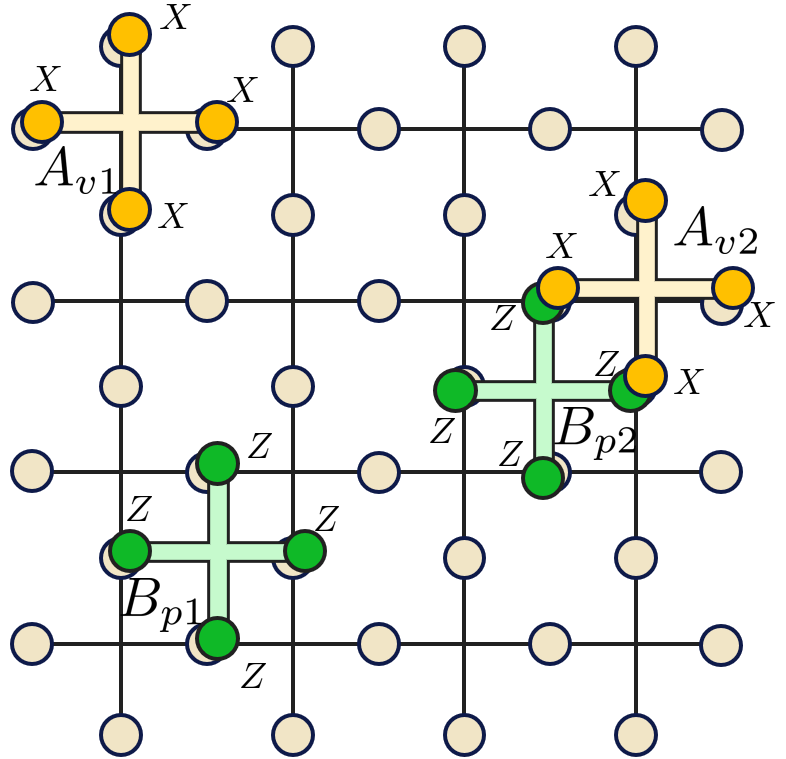
\includegraphics[width=0.3\columnwidth]{figures/chap4_toric_code_01.png}
    \caption{Toric code では量子ビットを各辺に配置し、頂点ごとに 頂点演算子 \(A_v\)、面ごとに 面演算子 \(B_p\) を定義する。
    隣接するような \(A_{v2}\) と \(B_{p2}\) の演算子は2本の辺を共有するため可換である。}
    \label{fig:chap4_toric_lattice_star}
\end{figure}

頂点に付随する \(A_v\) を頂点演算子、面に付随する \(B_p\) を面演算子と呼ぶ。
これらの演算子は互いに可換である。
実際、2つの 頂点演算子どうし、あるいは2つの 面演算子どうしは、
いずれもパウリ \(X\) 同士または \(Z\) 同士の積であるから可換である。
また、頂点演算子 \(A_v\) と 面演算子 \(B_p\) の組を考えると、
両者が共有する辺の本数は 0 本か 2 本である。
共有辺が 0 本ならば自明に可換であり、
共有辺が 2 本のときにも、各共有辺での反交換
\(XZ=- ZX\)
が2回現れるため、全体として符号は打ち消し合う。
したがって
\begin{equation}
    [A_v,B_p]=0
\end{equation}
が任意の \(v,p\) について成り立つ。

よって、これらの演算子をスタビライザー演算子として、符号空間を考えることができる。
Toric code の符号空間は、
全ての頂点 \(v\) と面 \(p\) に対して
\begin{equation}
    A_v\ket{\psi}=\ket{\psi},\qquad
    B_p\ket{\psi}=\ket{\psi}
\end{equation}
を満たす状態全体として定義される。
すなわち、
\begin{equation}
    \mathcal{C}
    =
    \qty{
        \ket{\psi}
        \mid
        A_v\ket{\psi}=\ket{\psi},
        B_p\ket{\psi}=\ket{\psi},
        \forall v,p
    }
\end{equation}
である。

また、これらのスタビライザーを用いると
\begin{equation}
    H=- \sum_v A_v- \sum_p B_p
\end{equation}
という可換局所ハミルトニアンを定義できる。
ここで各 \(A_v,B_p\) はいずれも固有値 \(\pm 1\) を持つので、
エネルギーが最小になるのは全ての頂点と面について
\begin{equation}
    A_v\ket{\psi}=\ket{\psi},\qquad
    B_p\ket{\psi}=\ket{\psi}
\end{equation}
が成り立つときである。
このハミルトニアンの基底状態空間は上で定義した符号空間 \(\mathcal{C}\) に一致する。
したがって、Toric code は量子誤り訂正符号であると同時に、
可換局所模型としても理解することができる。

\section{誤り鎖・論理演算子・シンドローム}

前節では、Toric code を格子上に定義された局所スタビライザー符号として導入し、
その符号空間を 頂点演算子と 面演算子の共通 \(+1\) 固有空間として定義した。
しかし、量子誤り訂正符号としてこの符号を理解するためには、
物理量子ビットに生じた誤りがどのように検出され、
その結果としてどのような論理自由度が残るのかを調べる必要がある。
Toric code の特徴は、これらの問いが格子上の図形を用いて
きわめて具体的に記述できる点にある。
まず誤りは辺に沿った鎖として表され、
さらに、シンドロームはその鎖の端点として読み取ることができる。
そのうえで、端点を持たない閉じた鎖のうち、
有限の領域の境界になっているものはスタビライザーとみなせる一方、
トーラスを一周するものはそれとは異なる役割を果たす。
このようにして、誤り、シンドローム、論理演算子の関係が
同じ幾何学的な言葉で統一的に記述される。
本節では、まず位相エラー \(Z(\gamma)\) から生じる誤り鎖とシンドロームの描像を導入する。
次に、閉じた鎖のうち有限の領域の境界になっているものが スタビライザー に対応することを見たうえで、
トーラスを一周するループから論理演算子を導入する。
最後に、前章で導入した \(N(S)/S\) の立場と結びつけながら
符号パラメータ \([[n,k,d]]\) を計算し、
復号問題が誤りそのものを当てる問題ではなく、
誤りの同値類を識別する問題として理解できることを見る。

まず、基準となる符号語の状態を用意する。
符号語はスタビライザーによる射影演算子を用いて任意の状態\(\ket{\psi}\)を射影することでえられる。
このToric codeにおけるスタビライザーは、頂点演算子 \(A_v\) と 面演算子 \(B_p\) である。
なので、これによる射影演算子は
\begin{equation}\begin{aligned}[b]
    \Pi_v &= \frac{1+A_v}{2},& \Pi_p &= \frac{1+B_p}{2}
\end{aligned}\end{equation}
である。
全ての頂点と面に対してこれらの射影演算子を掛けることで、符号空間への射影演算子となる。
なので基準となる符号語は
\begin{equation}
    \ket{\Omega}:= \prod_v \Pi_v\prod_p \Pi_p\ket{\psi}
    \propto \prod_v \frac{1+A_v}{2}\prod_p \frac{1+B_p}{2}\ket{\psi}
\end{equation}
のように表せる。
この状態は全ての \(A_v\) と \(B_p\) に対して固有値 \(+1\) を持つ。
実際、射影演算子\(\Pi_{v}\)に\(A_v\)を掛けると
\begin{equation}\begin{aligned}[b]
    A_v\Pi_v &= A_v\frac{1+A_v}{2} = \frac{A_v + A_v^2}{2} = \frac{A_v + 1}{2} = \Pi_v
\end{aligned}\end{equation}
\(\Pi_p\)に\(B_p\)を掛けると
\begin{equation}\begin{aligned}[b]
    B_p\Pi_p &= B_p\frac{1+B_p}{2} = \frac{B_p + B_p^2}{2} = \frac{B_p + 1}{2} = \Pi_p
\end{aligned}\end{equation}
となることを使うとわかる。
これより\(\ket{\Omega}\in\mathcal{C}\)と確認される。

以下では、この基準状態に生じる位相エラー \(Z(\gamma)\) の効果を調べることから始める。
まず、頂点\((v_1,v_2)\)を結ぶ1本の辺 \(e=(v_1,v_2)\) に沿ったエラーが入った状態
\begin{equation}
    Z(e)\ket{\Omega}
\end{equation}
を考える。
このパウリ \(Z(e)\) は、
その辺に接続する2つの頂点に対応する 頂点演算子とは反交換し、
それ以外の 頂点演算子とは可換である。
実際、式で書くと、
\begin{equation}\begin{aligned}[b]
    A_{v_1}Z(e)\ket{\Omega} &=- Z(e)A_{v_1}\ket{\Omega}=(-1)\times Z(e)\ket{\Omega},\\
    A_{v_2}Z(e)\ket{\Omega} &=- Z(e)A_{v_2}\ket{\Omega}=(-1)\times Z(e)\ket{\Omega}
\end{aligned}\end{equation}
であり、他の頂点 \(v\neq v_1,v_2\) については
\begin{equation}
    A_v Z(e)\ket{\Omega}=Z(e)A_v\ket{\Omega}=Z(e)\ket{\Omega}
\end{equation}
となる。
したがって、1つの位相エラー \(Z(e)\) は2つの頂点でのスタビライザー条件を破り、
その2点にシンドロームを生じさせる。

\begin{figure}[tb]
    \centering
    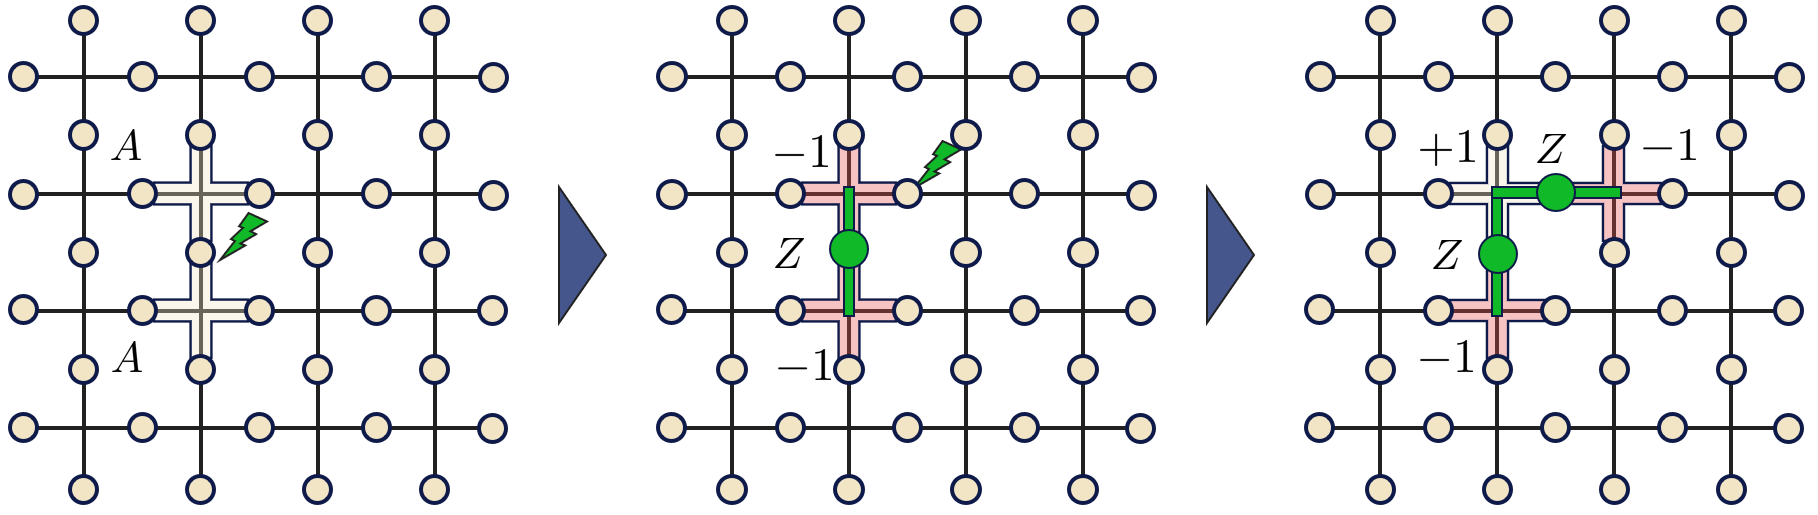
\includegraphics[width=0.8\textwidth]{figures/chap4_toric_code_02.png}
    \caption{位相エラーは格子上の \(Z\)- 鎖として表され、スタビライザーが\(A_v=-1\)となるシンドロームは鎖の端点に現れる。}
    \label{fig:chap4_toric_error_chain}
\end{figure}

次に、隣接する2本の辺 \(e_1=(v_1,v_3),e_2=(v_2,v_3)\) に位相エラーが入った状態
\begin{equation}
    Z(e_1+e_2)\ket{\Omega}
\end{equation}
を考える。
このとき、2本の辺が共有する頂点\((v_3)\)における頂点演算子\(A_{v_3}\)では
反可換になるヵ所が\(e_1, e_2\)の2か所存在するため、
\begin{equation}\begin{aligned}[b]
    A_{v_3}Z(e_1+e_2)\ket{\Omega} &= Z(e_1+e_2)A_{v_3}\ket{\Omega}=(+1)\times Z(e_1+e_2)\ket{\Omega}
\end{aligned}\end{equation}
のように、シンドロームが消える。
一方で、鎖の両端にある頂点では反交換が1回だけ残るため、
そこにのみシンドロームが現れる。
このことから、複数の辺にわたる位相エラーは格子上の鎖として表され、
シンドロームはその鎖の端点として理解できることがわかる。

一般に、辺の集合 \(\gamma\) に沿って位相エラーが入った状態は
\begin{equation}
    Z(\gamma)\ket{\Omega}
\end{equation}
のように書ける。
このとき鎖の内部にある頂点では反交換が偶数回起こるためシンドロームは消え、
端点にあたる頂点だけが\(A_v\)のスタビライザー条件の違反として残る。
したがって、位相エラーは格子上の \(Z\)-鎖として表され、
そのシンドロームは鎖の端点によって与えられる。

ここで重要なのは、同じシンドロームを与える誤り鎖は一般に一意ではないということである。
実際、同じ端点を持つ2つの鎖 \(\gamma,\gamma'\) を考えると、
それらの差 \(\gamma+\gamma'\) は端点を持たない閉じた鎖になる。
特に、その閉じた鎖がある領域 \(R\) の境界 \(\partial R\) として書けるとき、
\begin{equation}
    \gamma'=\gamma+\partial R
\end{equation}
である。
このとき対応する演算子は
\begin{equation}
    Z(\gamma') = Z(\gamma+\partial R)
    = Z(\gamma)Z(\partial R)
    = Z(\gamma)\prod_{p\in R} B_p
\end{equation}
と書ける。
したがって、\(\gamma\) と \(\gamma'\) は同じシンドロームを与えるだけでなく、
符号空間上では同じ作用を持つ。
この意味で、シンドロームが決めるのは誤り鎖そのものではなく、
境界を加える違いまで同一視した鎖の類である。

\begin{figure}[tb]
    \centering
    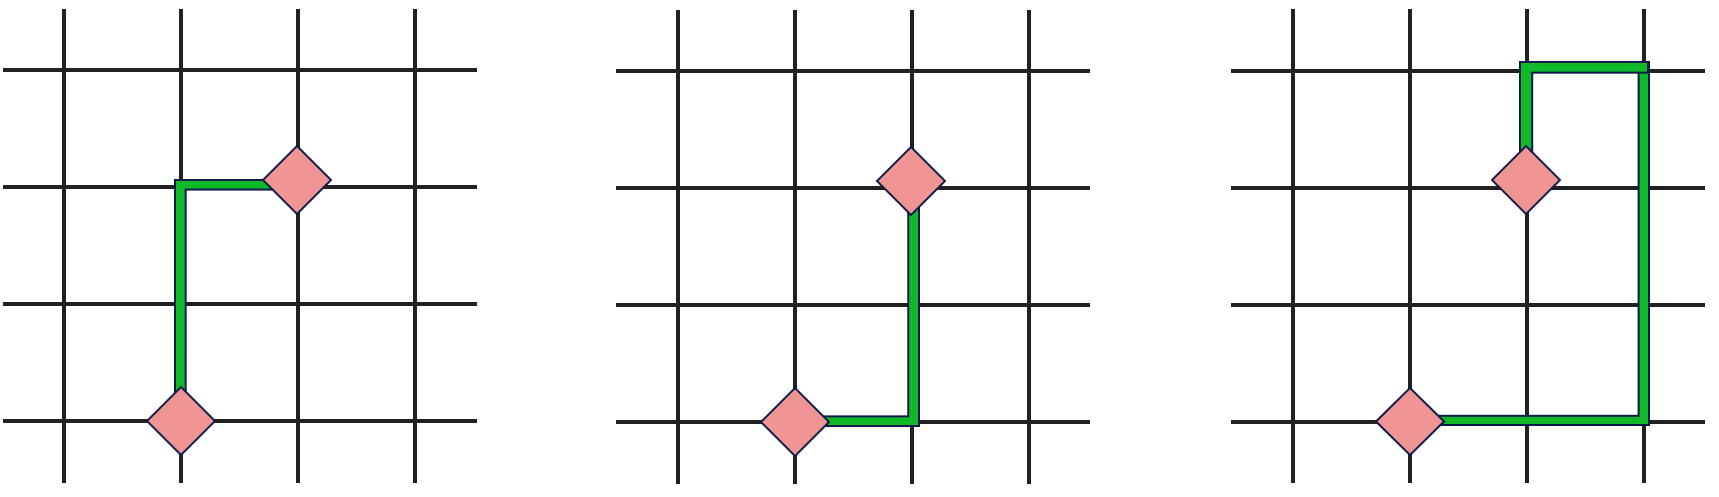
\includegraphics[width=0.8\textwidth]{figures/chap4_toric_code_03.png}
    \caption{同じシンドロームを与えるZ-鎖の例。
    ここでは辺にある量子ビットを省略して、頂点にあるスタビライザーが\(A_v=-1\)となるところのみ赤のひし形で示している。
    また、辺上にある緑の線はZ-鎖を表している。
    Z-鎖はスタビライザー\(B_p\)を加えることによって推移できる。
    つまりシンドロームからは鎖の端点以外の違いは識別できない。}
    \label{fig:chap4_toric_error_chain_equivalent}
\end{figure}

とくに、\(\gamma\) が閉じた鎖であるときには端点が存在しないため、
\(Z(\gamma)\ket{\Omega}\) は \(A_v\)によるスタビライザー条件の違反を生じない。
したがって、閉じた \(Z\)-鎖はシンドロームを持たない。
しかし、シンドロームを持たない閉じた鎖が全て同じ役割を果たすわけではない。
まず、\(\gamma\) が格子上のある有限の領域 \(R\) の境界 \(\partial R\) になっている閉ループである場合を考える。
このとき、その領域に含まれる 面演算子の積を取ると、
内部の辺では各 \(Z(e)\) が2回ずつ現れて打ち消し合い、
境界に沿う辺だけが1回ずつ残る。
したがって、\(\partial R\) に沿った閉ループ演算子は
\begin{equation}
    Z(\partial R)=\prod_{p\in R} B_p
\end{equation}
のように、その領域に含まれる 面演算子の積として書ける。
すなわち、この種の閉ループは スタビライザー の積にすぎない。
したがって、符号空間上では
\begin{equation}
    Z(\partial R)\ket{\psi}=\ket{\psi}
\end{equation}
が成り立ち、この種の閉ループは論理状態を変えない。

これに対して、\(\gamma\) がトーラスを一周してしまうような閉ループである場合には事情が異なる。
このようなループも閉じている以上シンドロームは生じないが、
もはやある有限領域の境界としては書けない。
したがって、そのような \(Z\)- ループは 面演算子の積では表せず、
スタビライザー 群には属さない。
それにもかかわらず、各 頂点演算子 \(A_v\) とは可換であり、
また 面演算子 \(B_p\) とも自明に可換である。
よって、そのような \(Z\)- ループは符号空間を保ちながら、
その内部で恒等的ではない作用をする演算子になっている。
\begin{figure}[tb]
    \centering
    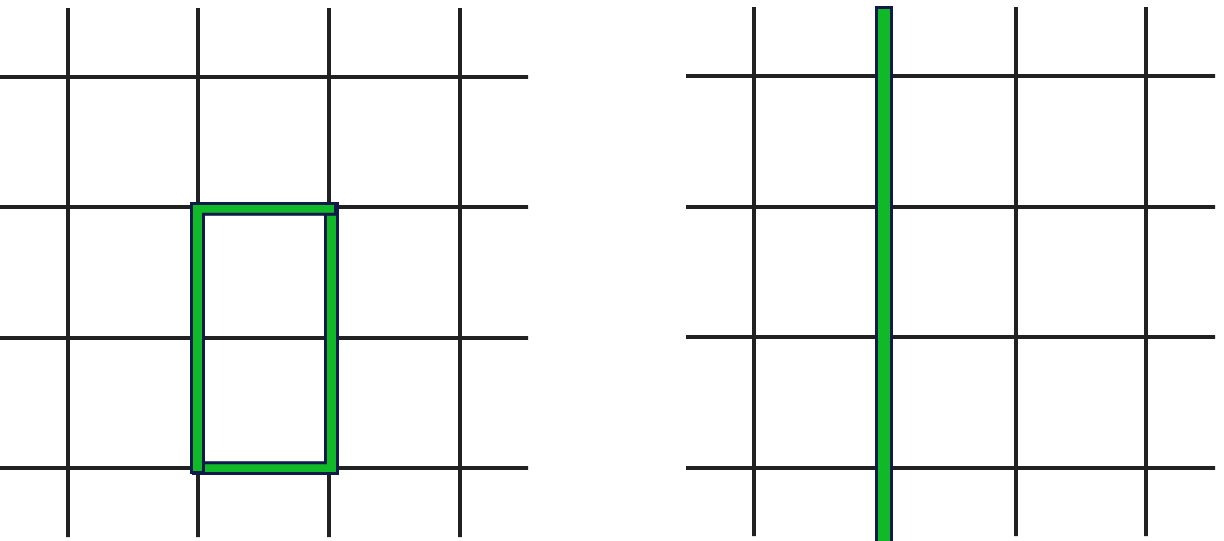
\includegraphics[width=0.54\textwidth]{figures/chap4_toric_code_04.png}
    \caption{Z-鎖がループ状になり端点がなくなったときの例。
    ここでは辺にある量子ビットを省略して辺上にある緑の線はZ-鎖を表している。
    実際にこのようなZ-ループのもと、頂点にあるスタビライザーの値を計算すると\(A_v=+1\)となり、シンドロームは検出されないのがわかる。
    左図は2つの四角の境界で表されるため、スタビライザー\(B_p\)の積で書けるのに対し、
    右図は周期境界を跨いでいるため、スタビライザーの積では書けない。}
    \label{fig:chap4_toric_error_loop}
\end{figure}

これは前章で導入した正規化群 \(N(S)\) の言葉で言えば、
全てのスタビライザーと可換であるから \(N(S)\) に属するが、
スタビライザー群 \(S\) 自身には属さない演算子になっているということである。
一般に、符号空間上で本質的な論理演算子は
正規化群をスタビライザー群で割った \(N(S)/S\) の元として分類される。
ここで見たトーラスを一周する \(Z\)- ループは、
ちょうどそのような \(N(S)/S\) の非自明な元の具体例になっている。
幾何学的には、これはループを境界だけの違いで同一視した類に対応しており、
この見方は次章でより系統的に扱うことになる。


同じ議論はパウリ\(X\)がかかるシフトエラーについても成り立つ。
そのために、まず双対格子を導入する。
これまで量子ビットを配置してきた格子を、ここでは元の格子と呼ぶことにする。
これに対して双対格子とは、元の格子の各面 \(p\) の中心を頂点 \(p^\ast\) とし、
隣接する面どうしに対応する頂点を辺 \(e^\ast\) で結んで得られる格子である。
このとき、双対格子の各辺 \(e^\ast\) は元の格子のちょうど1本の辺 \(e\) と交差しており、
両者の間には1対1の対応がある。
したがって、元の格子の辺に作用するパウリ \(X_e\) を、
それに対応する双対格子の辺 \(e^\ast\) に沿った演算子としてみなすことができる。

\begin{figure}[tb]
    \centering
    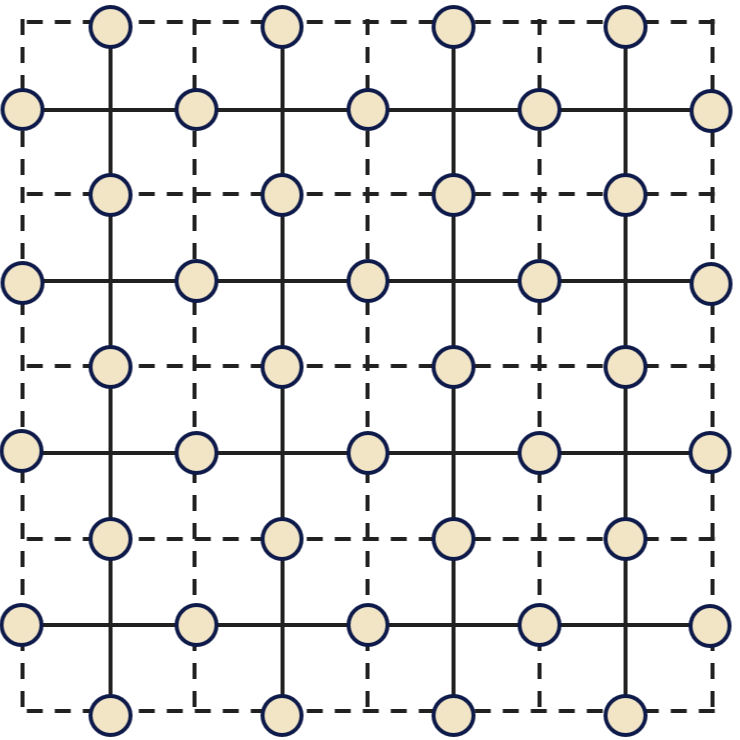
\includegraphics[width=0.25\columnwidth]{figures/chap4_dual_lattice.png}
    \caption{実線が元の格子、破線が双対格子を表している。
    双対格子は元の格子の面の中心を頂点とし、隣接する面の中心を結んだ格子である。
    双対格子の辺は元の格子のちょうど1本の辺と交差している。}
    \label{fig:chap4_toric_dual_lattice}
\end{figure}

いま、元の格子の1本の辺 \(e\) にシフトエラー \(X_e\) が生じたとする。
これに対応する双対格子の辺を \(e^\ast\) と書く。
この演算子は、その辺を境界に含む2つの 面演算子と反交換し、
それ以外の 面演算子とは可換である。
実際、辺 \(e\) を共有する2つの面を \(p_1,p_2\) とすると、
\begin{equation}
    B_{p_1}X_e\ket{\Omega}= -X_eB_{p_1}\ket{\Omega}= -X_e\ket{\Omega},
    \qquad
    B_{p_2}X_e\ket{\Omega}= -X_eB_{p_2}\ket{\Omega}= -X_e\ket{\Omega}
\end{equation}
であり、他の面 \(p\neq p_1,p_2\) については
\begin{equation}
    B_pX_e\ket{\Omega}= X_eB_p\ket{\Omega}= X_e\ket{\Omega}
\end{equation}
となる。
したがって、1つのシフトエラーは2つの面で面演算子のスタビライザー条件を破る。
この2つの面 \(p_1,p_2\) は双対格子では2つの頂点 \(p_1^\ast,p_2^\ast\) に対応しており、
\(X_e\) はそれらを結ぶ1本の双対辺 \(e^\ast\) に沿ったエラーとして表される。

一般に、双対格子上の辺の集合 \(\eta^\ast\) に沿って並んだ \(X\) 演算子の積を
\begin{equation}
    X(\eta^\ast):=\prod_{e^\ast\in\eta^\ast} X_e
\end{equation}
と書くことにする。
ここで \(e\) は双対格子の辺 \(e^\ast\) と交差する元の格子の辺を表している。
複数の辺にわたって \(X\) エラーが並ぶと、
内部では反交換が打ち消し合い、端点に対応する面だけにシンドロームが残る。
よって、シフトエラーもまた双対格子上の鎖 \(\eta^\ast\) として表され、
そのシンドロームは鎖の端点によって与えられる。
この見方を整理すると、元の格子の各頂点 \(v\) には双対格子の面 \(v^\ast\) が対応しているので、
元の格子で頂点に付いていた頂点演算子 \(A_v\) は双対格子では面 \(v^\ast\) に付いた面演算子のように見える。
一方、元の格子の面 \(p\) に付いていた面演算子 \(B_p\) は、
双対格子では頂点 \(p^\ast\) に付いた頂点演算子のように見える。
したがって、シフトエラー \(X\) に対する議論は、
位相エラー \(Z\) に対する議論を双対格子の上でそのまま言い直したものになっている。

\begin{figure}[tb]
    \centering
    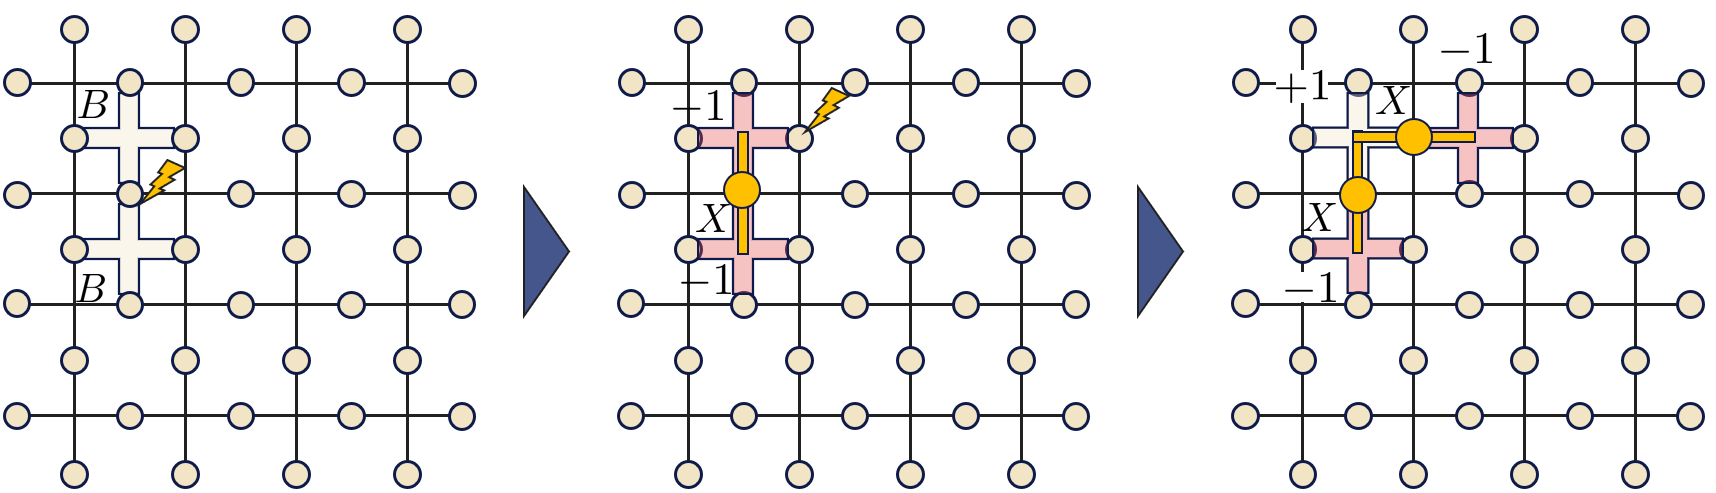
\includegraphics[width=0.8\textwidth]{figures/chap4_toric_code_05.png}
    \caption{シフトエラーは双対格子上の \(X\)-鎖として表され、そのシンドロームは鎖の端点に対応する面に現れる。}
    \label{fig:chap4_toric_x_chain}
\end{figure}

さらに、\(X\)-鎖 \(\eta^\ast\) が閉じたループになっている場合を考える。
このとき \(\eta^\ast\) は端点を持たないので、
対応する演算子 \(X(\eta^\ast)\) はどの面演算子 \(B_p\) の条件も破らない。
したがって、閉じた \(X\)-ループはシンドロームを持たない。

まず、\(\eta^\ast\) が双対格子上である有限の領域 \(R^\ast\) の境界
\(\partial R^\ast\) として書ける場合を考える。
このとき、その領域に含まれる双対格子の各面は
元の格子のある頂点 \(v\) に対応している。
対応する頂点演算子 \(A_v\) の積を取ると、
内部の辺では各 \(X_e\) が2回ずつ現れて打ち消し合い、
境界に沿う辺だけが1回ずつ残る。
したがって、
\begin{equation}
    X(\partial R^\ast)=\prod_{v^\ast\in R^\ast} A_v
\end{equation}
と書ける。
よって、双対格子上で有限の領域の境界になっている閉ループは、
頂点演算子の積にすぎず、符号空間上では自明に作用する。

これに対して、\(\eta^\ast\) がトーラスを一周するような閉ループである場合には、
それはシンドロームを持たないにもかかわらず、
もはや \(\partial R^\ast\) の形には書けない。
したがって、対応する \(X(\eta^\ast)\) は頂点演算子の積ではなく、
符号空間を保ちながらその内部で恒等的ではない作用をする。
このような \(X\)-ループは、\(Z\)-ループと同様に論理演算子の候補となる。

このように、元の格子上の \(Z\)- ループ \(Z(\ell)\) と、
双対格子上の \(X\)- ループ \(X(\eta^\ast)\) とは
ちょうど対をなして現れることがわかる。

以上より、論理演算子の候補として残るのは、
トーラスの2つの独立な方向に沿った \(Z\)-ループ2本と、
双対格子上の \(X\)-ループ2本である。
元の格子上の2つの独立な閉ループを \(\ell_1,\ell_2\) とし、
双対格子上の2つの独立な閉ループを \(\eta_1^\ast,\eta_2^\ast\) とすると、
これらはそれぞれ
\begin{equation}
    [Z(\ell_1)],\ [Z(\ell_2)],
    [X(\eta_1^\ast)],\ [X(\eta_2^\ast)]
\end{equation}
のような \(N(S)/S\) の非自明な元を与える。

同じ組に属する \([Z(\ell_i)]\) と \([X(\eta_i^\ast)]\) は、
元の格子と双対格子のループが1回だけ交差するように選ぶことができる。
そのため、それらに対応する代表元は、
ただ1つの辺でパウリ \(Z\) と \(X\) が反交換することから
\begin{equation}
    Z(\ell_i)X(\eta_i^\ast)=-X(\eta_i^\ast)Z(\ell_i)
    \qquad (i=1,2)
\end{equation}
を満たす。
一方、異なる組に属するループどうしは交差しないように選べるため、
\begin{equation}
    [Z(\ell_1),X(\eta_2^\ast)]=
    [Z(\ell_2),X(\eta_1^\ast)]=
    [Z(\ell_1),Z(\ell_2)]=
    [X(\eta_1^\ast),X(\eta_2^\ast)]=0
\end{equation}
である。
したがって、これらは2つの論理量子ビット上のパウリ演算子と同じ交換関係を満たしている。
そこで、これらを改めて
\begin{equation}
    \overline{Z}_1 := [Z(\ell_1)],\qquad
    \overline{Z}_2 := [Z(\ell_2)],\qquad
    \overline{X}_1 := [X(\eta_1^\ast)],\qquad
    \overline{X}_2 := [X(\eta_2^\ast)]
\end{equation}
と書くことにする。

よって、符号空間の基底は \(\overline{Z}_1,\overline{Z}_2\) の固有値によって
\begin{equation}
    \overline{Z}_1\ket{a,b}_L = (-1)^a \ket{a,b}_L,\qquad
    \overline{Z}_2\ket{a,b}_L = (-1)^b \ket{a,b}_L
    \qquad (a,b\in\{0,1\})
\end{equation}
のように選ぶことができる。
この基底に対して \(\overline{X}_1\) は1つ目の論理量子ビットを反転し、
\(\overline{X}_2\) は2つ目の論理量子ビットを反転する。
したがって、これらは2つの論理量子ビット上のパウリ演算子と同じ代数を実現しており、
Toric code には2つの独立な論理量子ビットが符号化されている。

\begin{figure}[tb]
    \centering
    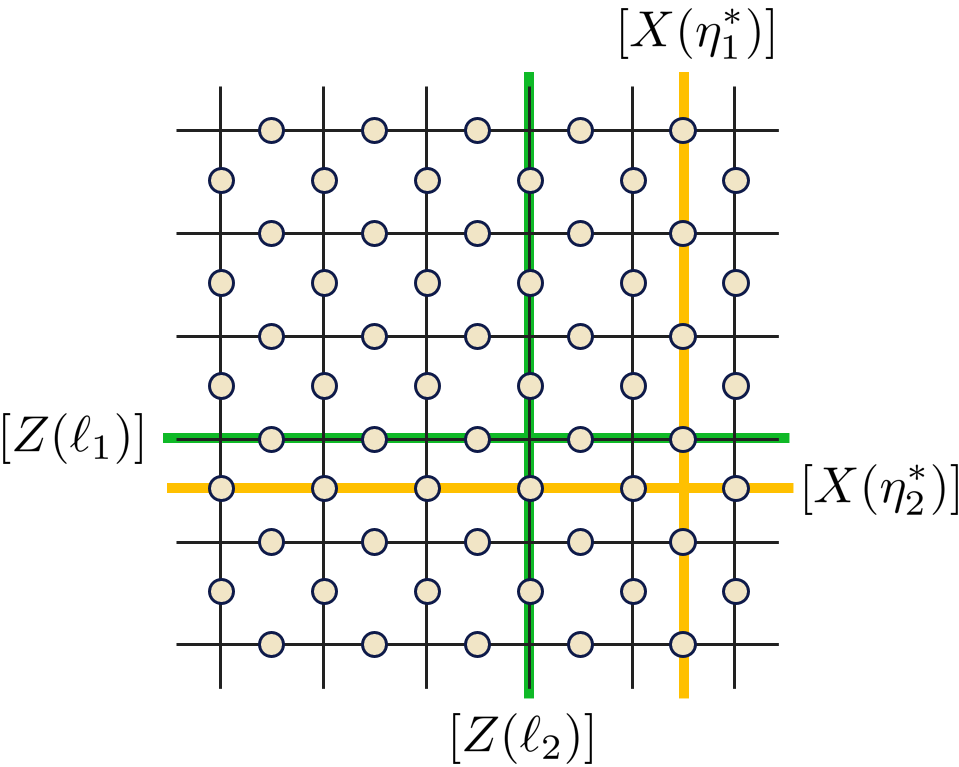
\includegraphics[width=0.4\columnwidth]{figures/chap4_toric_code_06.png}
    \caption{有限の領域の境界になっている閉ループは スタビライザー の積として書けるが、トーラスを一周する閉ループはそうではない。この違いが論理演算子の起源となる。}
    \label{fig:chap4_toric_loop}
\end{figure}

物理量子ビットの数 \(n\) は格子の辺の本数であり、
正方格子では水平方向と垂直方向にそれぞれ \(L_xL_y\) 本の辺があるため
\begin{equation}
    n=2L_xL_y
\end{equation}
である。
また、論理量子ビット数は
\begin{equation}
    k=2
\end{equation}
である。
さらに、符号距離 \(d\) はトーラスを一周するループのうち最短のものの長さで与えられるから、
\begin{equation}
    d=\min(L_x,L_y)
\end{equation}
となる。
とくに \(L_x=L_y=L\) の正方格子では
\begin{equation}
    [[n,k,d]]=[[2L^2,2,L]]
\end{equation}
である。

このように、Toric code では誤り鎖の端点がシンドロームとして観測され、
有限の領域の境界になっている閉ループは スタビライザー として自明であり、
トーラスを一周するループだけが論理演算子として残る。
したがって、復号において本質的なのは誤りの位置を完全に当てることではなく、
与えられたシンドロームに対して元の誤りと同じ同値類に属する回復演算を見つけることである。

\section{Toric code の復号と閾値}
前節では、Toric code における誤りが格子上の鎖として表され、
シンドロームがその端点として観測されることを見た。
また、復号において本質的なのは誤りの位置を完全に特定することではなく、
観測されたシンドロームに対して元の誤りと同じ同値類に属する回復演算を見つけることであると分かった。
したがって、Toric code の復号問題は、
端点の情報だけからもっともらしい誤り鎖の同値類を推定する問題として定式化される。

この節では、まず単純な確率的ノイズモデルのもとで
Toric code の復号問題を定式化する。
次に、物理エラー率に対して復号できるかどうかの閾値が存在することを説明する。
そしてこの閾値を決める問題が、統計力学のスピングラス模型と結びついていることを見る。

まず、最も単純なノイズモデルとして、各物理量子ビットに独立に位相エラー \(Z_e\) が確率 \(p\) で作用する状況を考える。
シフトエラーについても双対格子を考えると位相エラーと同様の議論が成り立つため、ここでは位相エラーだけを考えることにする。
このとき復号器が直接知ることができるのは、どの辺に誤りが起きたかではなく、
その結果として現れるシンドロームだけである。
しかし前節で見たように、同じシンドロームに整合する誤り鎖は一般に一意ではない。
実際、ある候補鎖に有限領域の境界を付け足してもシンドロームは変わらず、
しかも符号空間上では同じ作用を与える。
したがって、シンドロームが決めるのは誤り鎖そのものではなく、
境界の違いまで同一視した同値類である。

この点で、シンドロームからほぼ直接に誤り位置を読み取れる Shor 符号のような場合と比べると、
Toric code の復号では局所スタビライザーによる冗長性が本質的な役割を果たしている。
すなわち、同値類は代表元の取り方によらず定まる量であるにもかかわらず、
実際の復号器はその同値類に属する代表元を具体的に選ばなければならない。
さらにトーラス上では、候補鎖がどのホモロジー類に属するかによって
復号の成功と失敗が分かれる。
このように、同じシンドロームに対して多数の候補が存在し、
そのうちどのホモロジー類が正しいかを見分けなければならないという点に、
Toric code の復号の難しさがある。

物理エラー率 \(p\) を固定して系サイズ \(L\) を大きくしていったとき、
復号後に論理誤りが起こる確率がどのように振る舞うかは、
符号の性能を特徴づける重要な量である。
一般に \(p\) が十分小さい領域では、
系サイズを大きくするにつれて論理誤り率は下がっていく。
これに対して \(p\) が大きすぎると、
系サイズを大きくしても復号はうまく働かず、論理誤り率は下がらない。
この2つの振る舞いを分ける臨界的な誤り率が閾値（threshold）である。

この閾値をより構造的に理解するためには、
復号器が実際に何を比較しているのかを明確にする必要がある。
前節までに見たように、復号で本質的なのは個々の誤り鎖そのものではなく、
観測されたシンドロームに整合する候補のうち、どのホモロジー類がより尤もらしいかである。
したがって、閾値の問題は、各ホモロジー類に属する候補全体の重みが
ノイズ確率 \(p\) に応じてどのように競合するかを調べる問題に帰着される。
以下では、まずこのことをホモロジー類の事後確率最大化として定式化し、
これが双対格子上のランダム結合 Ising 模型の分配関数として表されることを見る。
そのために、観測されたシンドローム \(S\) に対し、まずそれと整合する 1 本の参照鎖 \(E_S\) を選ぶ：
\begin{equation}
    \partial E_S=S.
\end{equation}
すると、同じシンドロームを与える任意の候補鎖 \(E'\) は
\begin{equation}
    E'=E_S+C,\qquad \partial C=0
\end{equation}
と書ける。
すなわち、候補の曖昧さはすべて閉路 \(C\) を足す自由度に押し込められる。
さらにトーラス上では
\begin{equation}
    [C]\in H_1(T^2,\mathbb Z_2)\cong \mathbb Z_2\times \mathbb Z_2
\end{equation}
によって閉路のホモロジー類が 4 つに分類される。
よって、復号問題は「固定したシンドロームのもとで、どの候補鎖が最もありそうか」を問う問題から、
「どのホモロジー類が最もありそうか」を問う問題へと言い換えられる。

より具体的には、各ホモロジー類 \(h\in H_1(T^2,\mathbb Z_2)\) に対してその代表閉路 \(D_h\) を 1 本固定すると、
任意の候補鎖は
\begin{equation}
    E'=E_S+D_h+\partial m
\end{equation}
と表せる。
ここで \(\partial m\) はある面集合 \(m\) の境界であり、ホモロジー自明な閉路を表す。
したがって、
\begin{itemize}
    \item \(D_h\) はどのホモロジー類に属するかを表し、
    \item \(\partial m\) はその類の内部での局所的な揺らぎを表す。
\end{itemize}
復号器が比較すべきなのは、個々の候補鎖ではなく、各 \(h\) に属する候補全体の確率の和である。

各辺で独立に \(Z\) エラーが確率 \(p\) で起こるとする。
辺 \(\ell\) に対し
\begin{equation}
    n_E(\ell)=
    \begin{cases}
    1,& \ell\in E,\\
    0,& \ell\notin E
    \end{cases}
\end{equation}
を定めると、エラー鎖 \(E\) の確率は
\begin{equation}
    P(E)=\prod_{\ell} p^{n_E(\ell)}(1-p)^{1-n_E(\ell)}
\end{equation}
で与えられる。
ここで、ホモロジー類 \(h\) の事後確率とは、
その類に属する全ての候補鎖の事後確率を足し合わせたものである。
したがって、まず候補鎖 \(E'\) に対する事後確率を考える。
Bayes の定理より
\begin{equation}
    P(E'\mid S)=\frac{P(S\mid E')P(E')}{P(S)}
\end{equation}
である。
いま、固定したシンドローム \(S\) に整合する候補鎖だけを考えているので、
\(P(S\mid E')\) はそのような候補に対しては 1 であり、また \(P(S)\) は候補によらない定数である。
したがって、固定したシンドロームのもとでは
\begin{equation}
    P(E'\mid S)\propto P(E')
\end{equation}
が成り立つ。
次に、ホモロジー類 \(h\) の事後確率は、その類に属する全ての候補鎖の事後確率の和で与えられるから、
\begin{equation}
    P(h|S) = \sum_{E'\in h} P(E'|S)  \propto \sum_{E'\in h} P(E')
\end{equation}
となる。
さらに、\(h\) に属する任意の候補鎖は
\begin{equation}
    E'=E_S+D_h+\partial m
\end{equation}
と書けるので、
\begin{equation}
    P(h\mid S)
    \propto
    \sum_{m}P(E_S+D_h+\partial m)
\end{equation}
を得る。

最大尤度復号とは、この事後確率を最大にする \(h\) を選ぶことにほかならない：
\begin{equation}
    \hat h(S)=\arg\max_h P(h\mid S).
\end{equation}
したがって Toric code の復号とは、固定したシンドロームのもとでエラー鎖そのものを当てることではなく、
\emph{真のエラーが属するホモロジー類をベイズ推定すること}である。


ここまでで、復号の問題はホモロジー類 \(h\) の事後確率を最大にする問題へと言い換えられた。
次の目標は、この事後確率をスピン模型の分配関数として書くことである。
そのために、まず誤り鎖の描像を数式で扱いやすい形に書き換える。
すなわち、0/1 の辺占有を \(\pm1\) 変数に翻訳する。
参照鎖 \(E_S\) と閉路 \(C\) の各辺占有に対して
\begin{equation}
    \eta_\ell:=(-1)^{n_{E_S}(\ell)},
    \qquad
    u_\ell:=(-1)^{n_C(\ell)}
\end{equation}
と置く。
すると
\begin{equation}
    \eta_\ell=
    \begin{cases}
    +1,& \ell\notin E_S,\\
    -1,& \ell\in E_S,
    \end{cases}
    \qquad
    u_\ell=
    \begin{cases}
    +1,& \ell\notin C,\\
    -1,& \ell\in C
    \end{cases}
\end{equation}
であり、
\begin{equation}
    \eta_\ell u_\ell=(-1)^{n_{E_S}(\ell)+n_C(\ell)}=(-1)^{n_{E'}(\ell)}
\end{equation}
は最終的な候補鎖 \(E'=E_S+C\) の辺占有を表す。
したがって
\begin{equation}
    n_{E'}(\ell)=\frac{1-\eta_\ell u_\ell}{2}
\end{equation}
であり、候補鎖の確率は
\begin{equation}
    P(E')
    \propto
    \prod_\ell
    \left(\frac{p}{1-p}\right)^{(1-\eta_\ell u_\ell)/2}
\end{equation}
と書ける。
ここで
\begin{equation}
    e^{-2K}=\frac{p}{1-p},
    \qquad
    K=\frac12\log\frac{1-p}{p}
\end{equation}\footnote{
後で見るように、この \(K\) は双対格子上のランダム結合 Ising 模型の逆温度に対応する。
その際、disorder に由来する結合定数の確率分布を表す \(p\) と、
熱浴との相互作用に由来する温度\(K=\beta J\)は本来独立な量であるが、
復号問題に対応するのは \(e^{-2K}=p/(1-p)\) を満たす特別な線に限られる。
この線は西森線と呼ばれる。}
と置けば、
\begin{equation}
    P(E') \propto \exp(K\sum_\ell \eta_\ell u_\ell)
\end{equation}
となる。

これらの変数は候補鎖の重みを辺ごとに書くには便利であるが、
閉路 \(C\) の幾何学的な構造そのものを見通しよく表しているわけではない。
とくに、ホモロジー自明な閉路は面集合 \(m\) の境界 \(\partial m\) として表されるので、
辺の変数よりも面の変数で記述した方が自然である。

そこで次に、ホモロジー自明な閉路を双対格子上の \(\pm1\) 変数で表すことを考える。
双対格子の各頂点 \(i\) に \(\sigma_i=\pm1\) を置くと、隣接する双対格子の頂点 \(i,j\) に対し
\begin{equation}
    u_{ij}=\sigma_i\sigma_j
\end{equation}
と書ける。
これは、\(\sigma\) をある領域の内部で反転させたとき、その境界に沿って \(\sigma_i\sigma_j=-1\) が現れることに対応している。
すなわち、\(\sigma\) の符号が変化する境界が元の格子上の閉路 \(C\) を表す。
この意味で辺\(\ell = (i,j)\)の変数 \(u_{ij}\) は、辺 \(\ell\) が閉路 \(C\) に含まれるかどうかを表す指示関数になっている。
したがって、ホモロジー自明な閉路 \(C\) に対しては
\begin{equation}
    u_{\ell} = u_{ij}=
    \begin{cases}
    +1,& \text{その辺が閉路に含まれない},\\
    -1,& \text{その辺が閉路に含まれる}
    \end{cases}
\end{equation}
となる。

ただし、\(\sigma_i\sigma_j\) と書けるのはあくまでホモロジー自明な閉路に対してである。
トーラス上には非自明な巻き付き閉路があるので、ホモロジー類 \(h\) の情報は別に入れなければならない。
そのため、各 \(h\) に対して固定背景 \(\bar u_{ij}^{(h)}\) を導入し、
\begin{equation}
    u_{ij}^{(h)}=\bar u_{ij}^{(h)}\sigma_i\sigma_j
\end{equation}
と書く。
ここで \(\bar u^{(h)}\) はホモロジー類 \(h\) を指定するねじれを表しており、
トーラスを一周する非自明な閉路に沿った欠陥線とみなしてよい。
すなわち、\(u_{ij}^{(h)}\) はホモロジー類 \(h\) に属する候補鎖が、
辺 \(\ell=(i,j)\) を通るかどうかを表す \(\pm1\) 変数になっている。
先ほど得た候補鎖の重み
\begin{equation}
    P(E')
    \propto
    \exp\left(
    K\sum_\ell \eta_\ell u_\ell
    \right)
\end{equation}
に、この \(u_\ell=u_{ij}^{(h)}\) を代入すると、
各ホモロジー類ごとの重みは双対格子上の \(\sigma\) 配置についての和として表される。
したがって候補のホモロジー類ごとの重みは
\begin{equation}
    Z(h\mid S)
    =
    \sum_{\{\sigma\}}
    \exp\left(
    K\sum_{\langle ij\rangle}
    \eta_{ij}\,\bar u_{ij}^{(h)}\,\sigma_i\sigma_j
    \right)
\end{equation}
で与えられる。
この形は双対格子上の \(\pm J\) ランダム結合 Ising 模型
\begin{equation}\begin{aligned}[b]
    H(\{\sigma\}\mid h,S)
    &:=-\sum_{\langle ij\rangle} J_{ij}(h\mid S)\,\sigma_i\sigma_j,\\
    J_{ij}(h\mid S)&:=K\eta_{ij}\bar u_{ij}^{(h)}
\end{aligned}\end{equation}
の分配関数そのものである。
\(\eta_{ij}=+1\) の辺は強磁性的な結合、\(\eta_{ij}=-1\) の辺は反強磁性的な結合に対応する。
したがって参照鎖 \(E_S\) が通る辺が、凍結したランダム結合として disorder を与えることになる。

以上の写像により、各ホモロジー類の事後確率は
\begin{equation}
    P(h\mid S)
    =
    \frac{Z(h\mid S)}{\sum_{h'}Z(h'\mid S)}
\end{equation}
と書ける。
ここで \(K\) は、統計力学でよく用いられる無次元結合定数であり、
通常の記法では \(K=\beta J\) と書かれる量にあたる。

この段階で、復号問題は次の形に読み替えられたことになる：
\begin{quote}
固定したシンドロームのもとで、4 つのホモロジー類に対応する
ランダム結合 Ising 模型の分配関数 \(Z(h\mid S)\) を比較し、最も重い類を選ぶ。
\end{quote}
言い換えれば、Toric code の最大尤度復号は、ランダム結合 Ising 模型の
ねじれた 4 つのホモロジー類の重みを比較する問題である。

各ホモロジー類の自由エネルギー
\begin{equation}
    F(h\mid S):=-\frac{1}{K}\log Z(h\mid S)
\end{equation}
を導入すると、
\begin{equation}
    P(h\mid S)
    =
    \frac{e^{-KF(h\mid S)}}{\sum_{h'}e^{-KF(h'\mid S)}}
\end{equation}
となる。
したがって
\begin{equation}
    -\frac{1}{K}\log P(h\mid S)
    =
    F(h\mid S)+\text{const.}
\end{equation}
であり、定数を除けば事後確率の比較は自由エネルギーの比較に等しい。
ゆえに
\begin{equation}
    \hat h(S)=\arg\max_h P(h\mid S)=\arg\min_h F(h\mid S)
\end{equation}
である。
すなわち、最大事後確率復号は、最小自由エネルギーを与えるホモロジー類を選ぶことに等価である。

ここで問題の見方がもう一段変わる。
もともと復号は「もっとも確からしいエラーを選ぶ問題」であったが、
いまやそれは「ねじれを入れた 4 つのホモロジー類のうち、自由エネルギーが最も低いものを選ぶ問題」として理解される。
この読み替えが、復号閾値と統計力学的相転移とを結びつける核心である。

% ランダム結合 Ising 模型自体は、一般には disorder 濃度 \(p\) と温度 \(T\) を独立に動かす 2 変数の模型である。
% しかし復号問題では、温度に対応するパラメータは物理温度ではなく、復号器が候補鎖に与える重み付けを表している。
% もし復号器が真のノイズ率 \(p_*\) とは異なる率 \(q\) を仮定して候補を重み付けするなら、
% \begin{equation}
%     e^{-2K_q}=\frac{q}{1-q}
% \end{equation}
% に対応する別の線で事後確率を評価していることになる。
% これに対し
% \begin{equation}
%     q=p_*
% \end{equation}
% であるとき、すなわち復号器が真の生成分布を正しく仮定しているときに限り、
% 統計力学模型の Gibbs 分布は元の復号問題の真の事後確率分布に一致する。
% この意味で 西森線とは、単なる便利な置換ではなく、
% \begin{quote}
% disorder を生成した確率法則と、復号器が用いる重み付けとが一致している線
% \end{quote}
% である。
% したがって、最大尤度復号の閾値を問うなら、相図全体ではなく 西森線上でホモロジー類の自由エネルギー差がどう振る舞うかを見ればよい。

% このことを踏まえて、実際の復号閾値は西森線上での自由エネルギー差の振る舞いによって決まる。
そこで、自明なホモロジー類を \(h=0\) とし、非自明なホモロジー類との自由エネルギー差を
\begin{equation}
    \Delta F_h:=F(h\mid S)-F(0\mid S)
    \qquad (h\neq 0)
\end{equation}
と書く。
物理的には、\(\Delta F_h\) はトーラスを一周する非自明な domain wall を挿入する自由エネルギーコストと解釈できる。

エラー率\(p\)が小さい、つまり\(K=\beta J \gg 1\)の低温の秩序相では、大域的な非自明 domain wall を入れるには系サイズに比例するコストが必要である。
したがって
\begin{equation}
    \Delta F_h\sim c_h L
    \qquad (h\neq 0)
\end{equation}
となり、熱力学極限 \(L\to\infty\) で非自明なホモロジー類の重みは指数的に抑圧される：
\begin{equation}
    P(h\neq 0\mid S)\sim e^{-K_p c_h L}\to 0.
\end{equation}
この場合、事後確率は正しいホモロジー類に集中し、論理誤り率は 0 に近づく。

これに対してエラー率の大きい、つまり\(K=\beta J \ll 1\)の高温の無秩序相では、大域的 domain wall を入れる自由エネルギーコストはもはや系サイズに比例せず、せいぜい \(O(1)\) にしかならない。
すると複数のホモロジー類が熱力学極限でも競合し、事後確率は 1 つの類に集中しない。
その結果、論理誤り率が有限に残る。
したがって復号閾値とは、
\begin{quote}
% 西森線上で、
非自明なホモロジー類を抑圧していた大域的自由エネルギー障壁が消える点
\end{quote}
である。
言い換えれば、秩序相ではホモロジー類の自由エネルギー差が論理情報を支える秩序として働くが、
無秩序相ではその秩序が失われ、異なるホモロジー類を自由エネルギーで区別できなくなる。

以上より、2 次元 Toric code の理想シンドローム測定のもとでの独立誤りに対する誤り閾値がどれくらいの確率かという問題は、
双対格子上の 2 次元 \(\pm J\) ランダム結合 Ising 模型における相転移温度を調べる問題へと帰着する。
そしてその復号閾値は、この模型の相図において 西森線と強磁性相・常磁性相境界の交点として与えられる。
この点は数値的によく研究されており、
\begin{equation}
    p_{\mathrm{th}}\simeq 0.1094 \approx 10.9\%
\end{equation}
が得られている。
したがって、2 次元 Toric code の最大尤度復号の閾値としてしばしば引用される「約 \(11\%\)」とは、
まさにこの西森点の値に対応している。

最後に強調しておくと、この \(11\%\) という数値はいつでも成り立つ普遍的な値ではない。
ここで仮定したのは、
\begin{itemize}
    \item 2 次元 Toric code、
    \item 各量子ビットに独立に誤りが入る雑音モデル、
    \item シンドローム測定誤りを含まない状況、
    \item \(X\) と \(Z\) を独立に扱う CSS 的状況、
    \item 最大尤度復号
\end{itemize}
というかなり特定の設定である。
たとえば復号器を MWPM に変えれば閾値は少し変わり、シンドローム測定誤りまで入れれば対応する統計力学模型そのものが変わる。
それでもなお、復号問題をホモロジー類のベイズ推定として定式化し、それを 西森線上の自由エネルギー比較として読むという見方は、
Toric code の閾値の意味を理解するうえで最も基本的な枠組みである。

\end{document}
